\chapter{The Commonwealth should prioritise a small number of national reforms}\label{chap:few-reforms}

\Chapref{chap:Commonwealth-conditions} highlighted the dangers of using new federal funding conditions to drive education reform. This chapter argues that the Commonwealth should pursue a small number of reforms (at most) that have a high chance of success. It outlines criteria that should be used to assess potential Commonwealth reforms.

\section{Screen reforms through a prioritisation process}\label{sec:screen-reforms}

Developing an integrated approach for even one major reform effort is hard work. Trying to implement a long list of reforms means efforts are likely to be too thinly spread to improve practice in the classroom -- the ultimate goal.

\begin{figure}
\caption{The Commonwealth should intervene only if a reform proposal meets these three criteria}\label{fig:criteria-to-determine-if-proposed-reforms}
\includegraphics[page=3]{charts/GonskiReportCharts.pdf}
\end{figure}

We propose a prioritisation framework with three criteria for identifying a small number of reforms with a high chance of success (see \Vref{fig:criteria-to-determine-if-proposed-reforms}). The three criteria are: 

\begin{itemize}
    \item Is it a good idea? There should be strong evidence that the core concept of the proposal will have a big and positive impact on student outcomes, and can address a big problem in the Australian system in reasonable time and at reasonable cost. 
    \item Can government make it happen? There should be expert consensus that government intervention can make a difference, with the right system settings, policies and/or programs to help bring the idea into practice.
    \item Will Commonwealth intervention help? The idea must be amenable to Commonwealth oversight and monitoring. Benefits such as national scale, filling a gap, and policy consistency, should be weighed against costs such as duplication, displacement of state priorities, policy incoherence, and red tape. State `buy-in' to the problem and solution is critical for the collaborative effort to work.   

\end{itemize}



\section{Conditions are often costly and hard to impose}\label{sec:conditions-fall-down}

Many proposed Commonwealth controls may look like a good idea in theory; that is, they may meet the conditions set out in criterion 1 (Is it a good idea?). But most tend to fall down on criterion 2 (Can government make it happen?) and criterion 3 (Will Commonwealth intervention help?). In particular, it is difficult for the Commonwealth\space government to adequately monitor the controls from Canberra, and there are confusion and costs from an extra layer of government involvement. 

Commonwealth requirements that simply mandate a specific `evidence-based practice' are unlikely to lead to much practical change. State and territory governments can rarely just flick a switch to implement a Commonwealth directive.

The Commonwealth may not know that elements in the delivery chain might be missing at the state level. Simply requiring one new initiative is unlikely to deliver change if other state-level policies are not aligned to support it.

\subsection{The `requiring explicit teaching in schools' example}\label{subsec:explicit-teaching}

In its Quality Outcomes Quality Schools 2016 strategy, the Commonwealth Government said it intended to require \textit{``explicit teaching in schools''}.\footcite{2016AustralianGovernmentQualitySchoolsQualityOutcomes} While `explicit teaching' is strongly backed by evidence (although not as an exclusive strategy), it would be a poor policy choice for the Commonwealth.

First, there is not yet any common understanding of what `explicit teaching' would involve, or exactly how different it would be from current practice.

Second, state governments are unlikely to have the right mix of policies and programs to help teachers switch to `explicit teaching'. States do not have a good track record in scaling evidence-based practice. For example, the right professional learning, school structures, accountability processes, and incentives all need to be in place.

Third, it is not clear that the Commonwealth is best-placed to lead this change. It would be difficult, for example, for the Commonwealth to independently monitor and verify changes in teaching practice, given little data is collected on teaching practices in schools.

Finally, there would be costs arising from the confusion in adding a federal policy at odds with state policies. A federal requirement mandating a certain practice would be inconsistent with the policy approach of most states, which is to devolve decisions on pedagogy to schools.

Regardless of whether mandating `explicit teaching' is a good policy, enforcing it from the Commonwealth level would create policy incoherence and could create confusion in regions and schools. 

